\chapter{Introduction}
This chapter describes the design and development of the LAB.E.S platform. \\
It emphasizes the strategic decisions and critical actions necessary to convert the laboratory's requirements into a functioning, high-performance platform.
First, the solution's overall layout is detailed, emphasizing its modular and scalable character, which allows harmonic integration of the various components while satisfying the criteria for flexibility and sustainability.
The chapter also describes the database structure, which was built to effectively manage data flows in real time while ensuring the consistency and security of the laboratory's important information.
On a technical level, it describes what steps were taken to construct the frontend and backend. The frontend, built on Figma's UX/UI models, provides an intuitive, high-performance user experience powered by current technologies such as React. Meanwhile, the backend relies on strong, secure services to ensure data processing and interchange across system components.\\
This introduction gives a basic overview which establishes the groundwork for the chapter, which delves into every technical and conceptual element needed in building a solution customized to the laboratory's unique requirements.

\section{Project Architecture Design}

\subsection{System Overview}
The LAB.E.S platform was built using a multi-tier architecture to ensure modularity, scalability, and maintainability. The system is divided into three primary layers:
\begin{itemize}
    \item \textbf{Frontend Layer}: Developed using ReactJS for a responsive and dynamic user interface.
    \item \textbf{Backend Layer}: Built with ASP.NET Core, providing RESTful APIs for communication with the frontend.
    \item \textbf{Data \& Communication Layer}: Handles real-time data exchange using MQTT and stores data in a relational database (SQL Server).
\end{itemize}


\subsection{Microservices Approach}
A microservices architecture was adopted to decouple various system functionalities, allowing independent deployment and scaling of each component. This architecture ensures that the platform remains robust and adaptable as new features are added.
\clearpage


\section{Frontend Development}

\subsection{UI/UX Design Using Figma}
The design of the user interface was initially conceptualized on Figma, focusing on user experience and intuitive navigation. The goal was to create a streamlined interface for laboratory personnel to monitor equipment and data efficiently.

\begin{figure}[H]
    \centering
    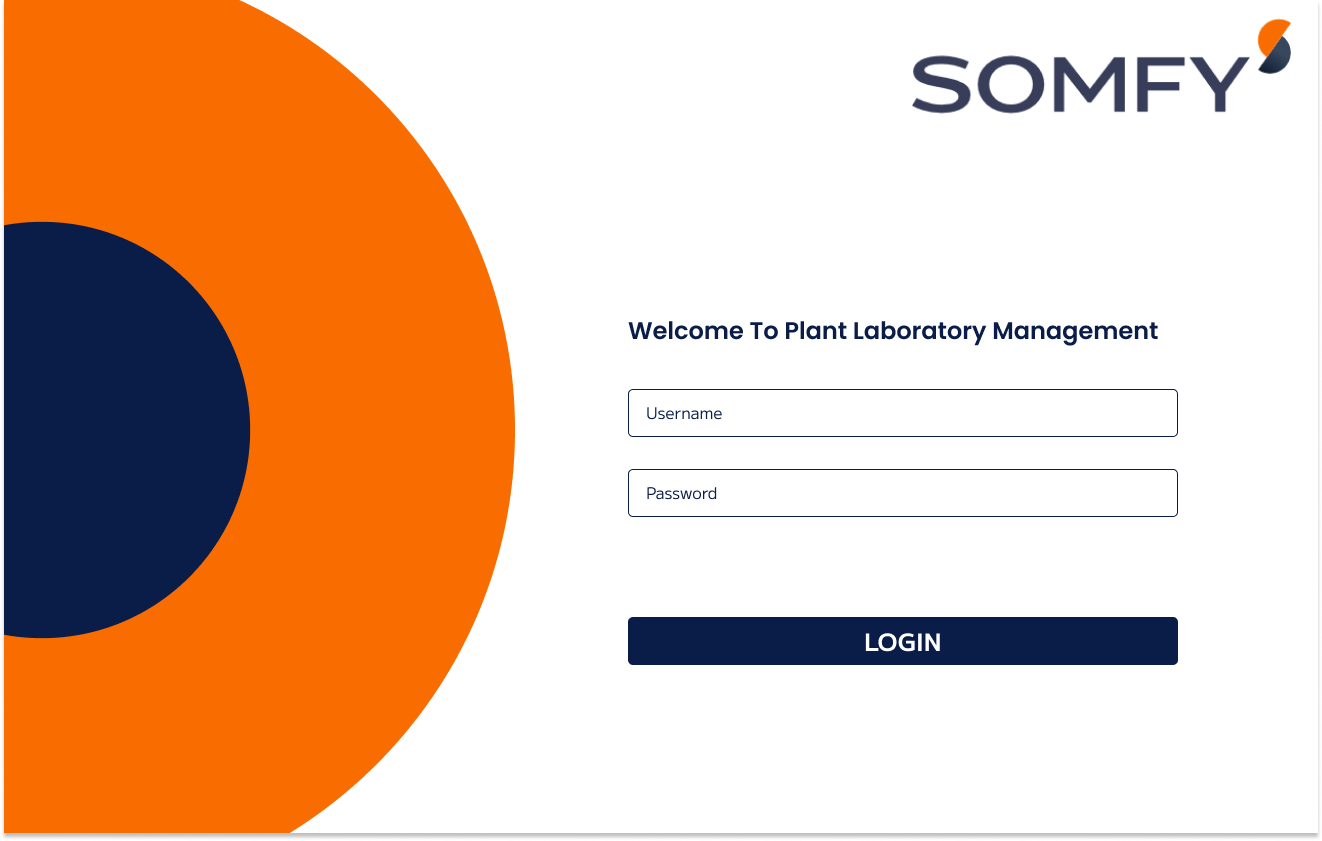
\includegraphics[width=1\textwidth]{chapters/3/img/10.png}
    \caption{cp 242-1 LEAN}
    \label{fig:campus}
\end{figure}

BLABALALALALNA LNNNLLALD

\begin{figure}[H]
    \centering
    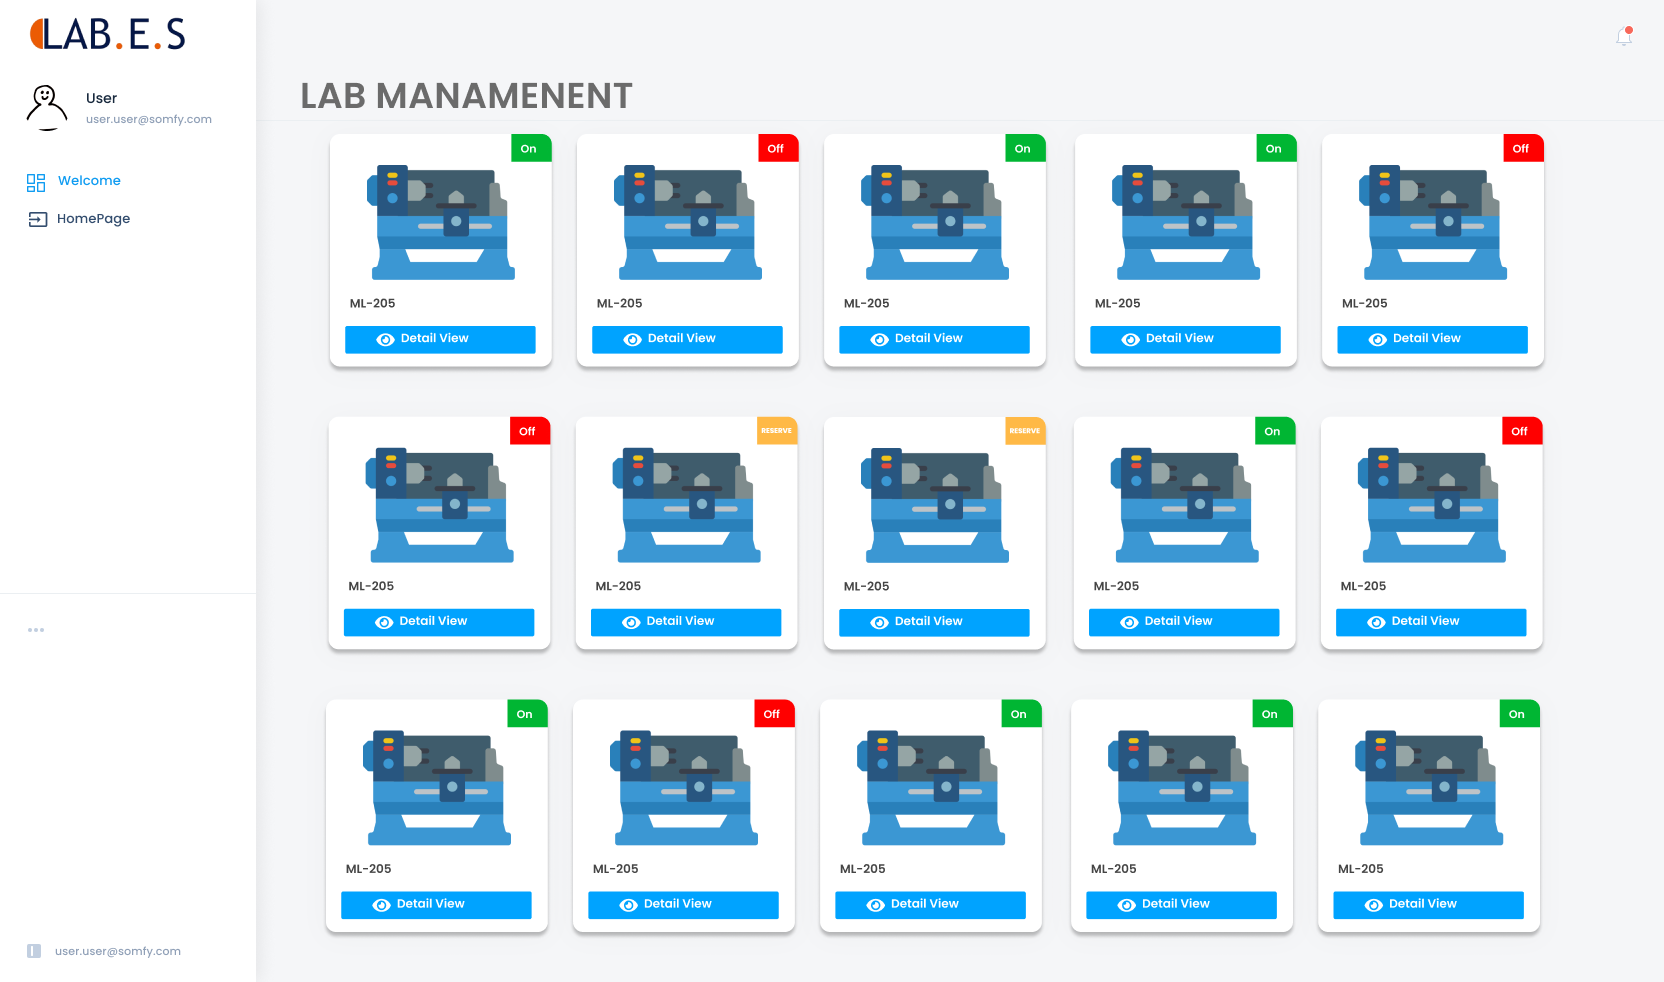
\includegraphics[width=1\textwidth]{chapters/3/img/12.png}
    \caption{cp 242-1 LEAN}
    \label{fig:campus}
\end{figure}



\subsection{ReactJS Implementation}
The frontend was implemented using ReactJS, leveraging its component-based architecture. This allowed for the creation of reusable components, reducing development time. Key features include:
\begin{itemize}
    \item \textbf{Real-Time Data Visualization}: Dynamic dashboards to monitor lab operations.
    \item \textbf{Interactive Forms}: Efficient data entry and equipment management.
    \item \textbf{Responsive Design}: Ensuring compatibility across devices, from desktops to tablets.
\end{itemize}


\begin{figure}[H]
    \centering
    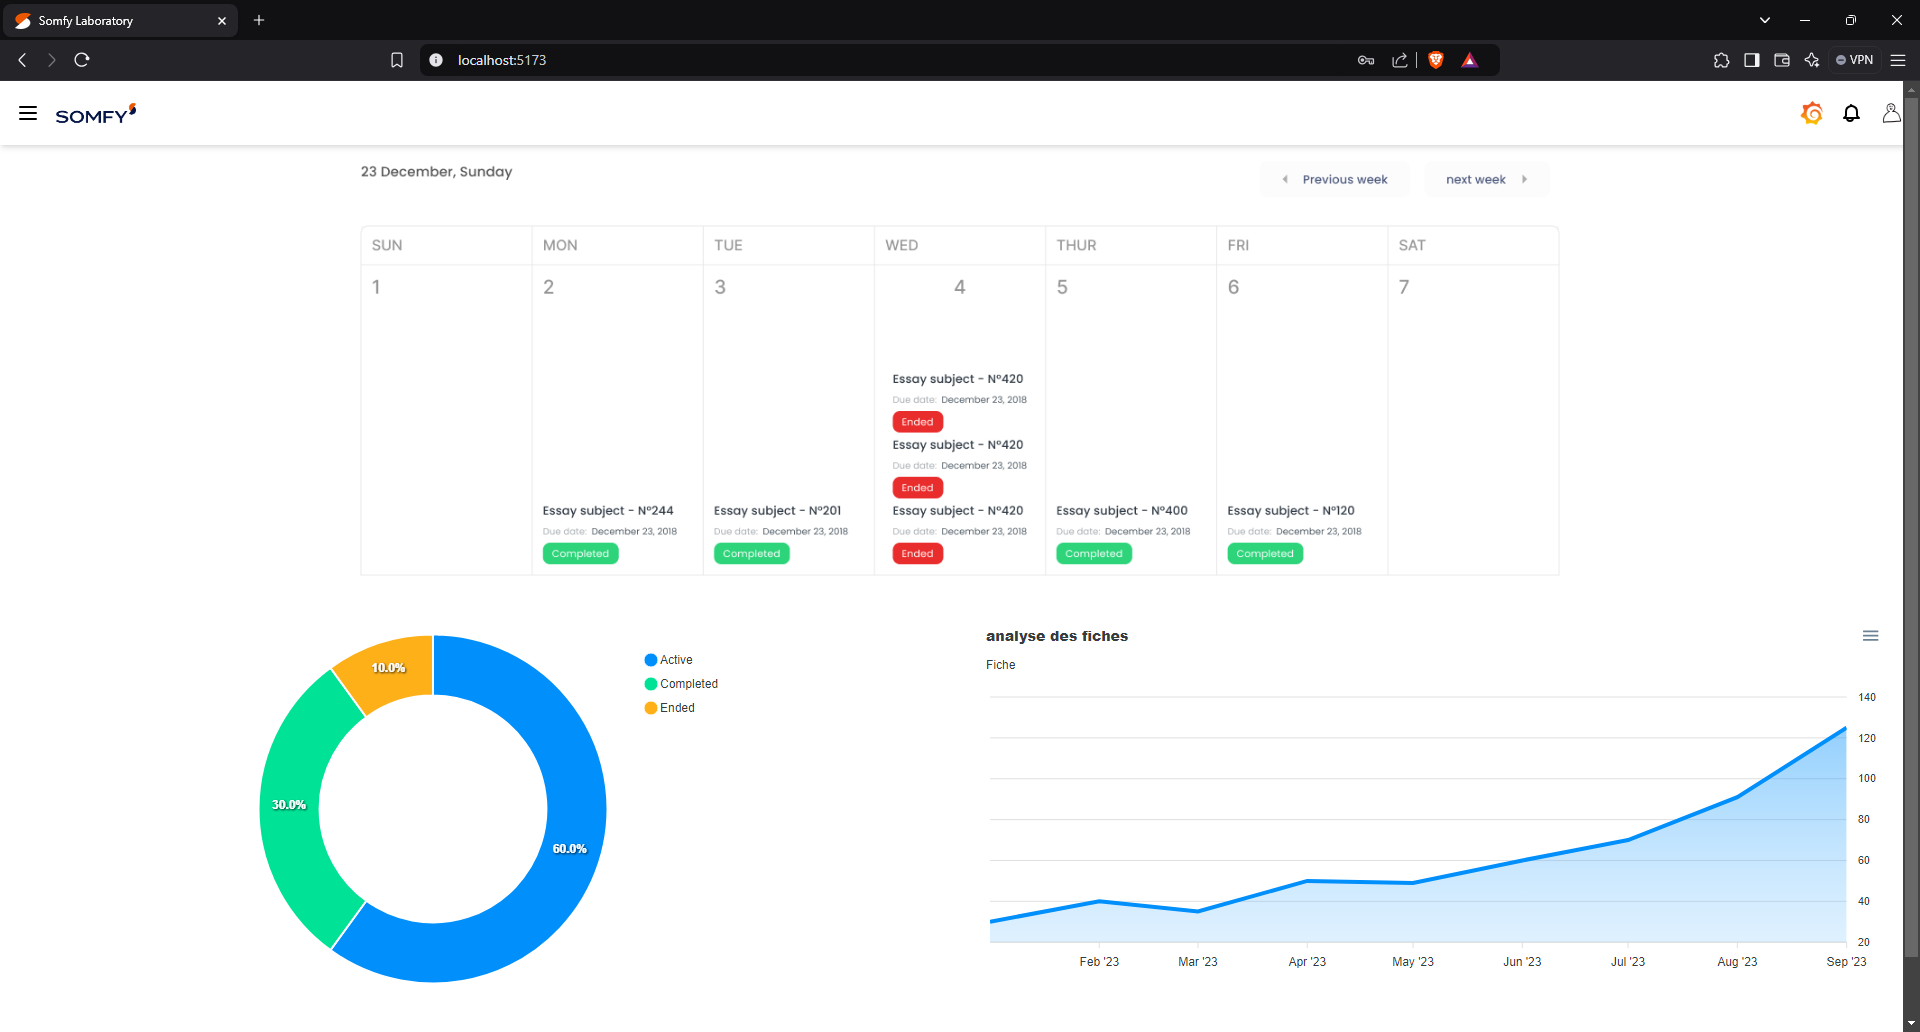
\includegraphics[width=1\textwidth]{chapters/3/img/2.png}
    \caption{cp 242-1 LEAN}
    \label{fig:campus}
\end{figure}


\begin{figure}[H]
    \centering
    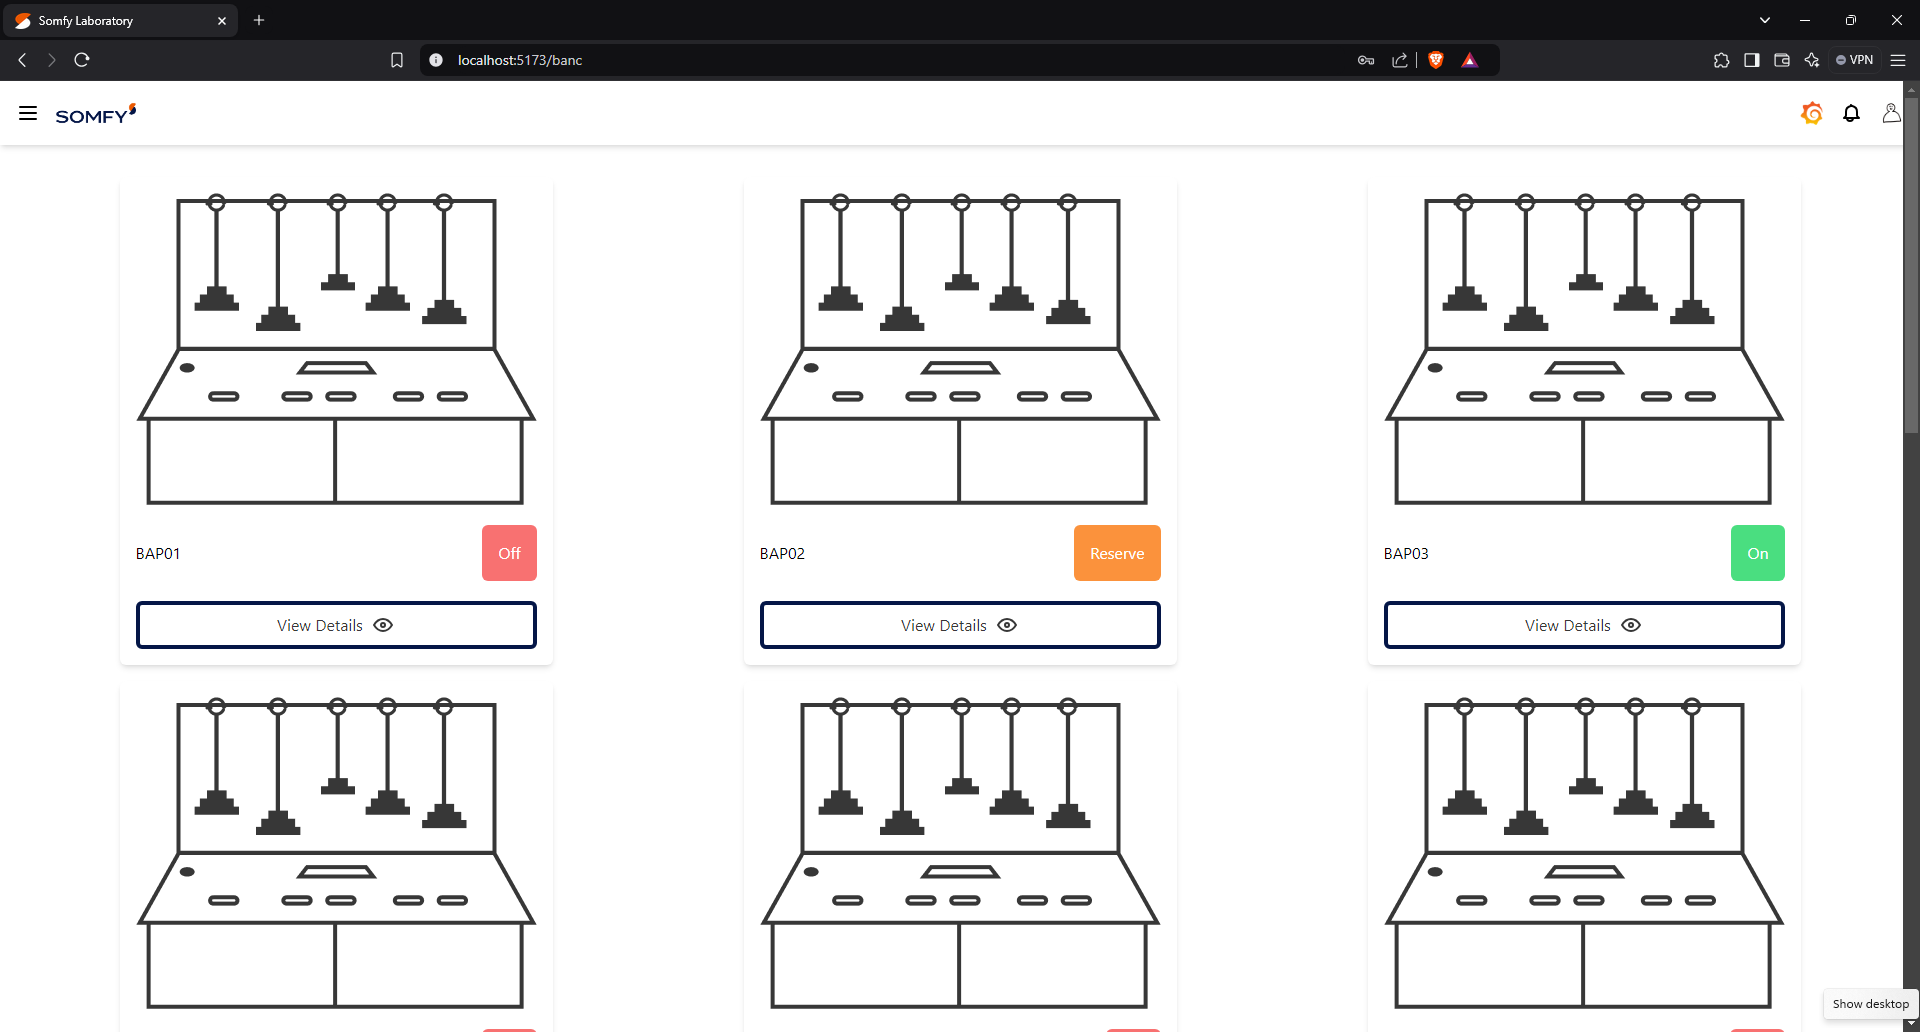
\includegraphics[width=1\textwidth]{chapters/3/img/6.png}
    \caption{cp 242-1 LEAN}
    \label{fig:campus}
\end{figure}










\section{Backend Development}

\subsection{Backend Architecture with ASP.NET Core}
The backend services were developed using ASP.NET Core, which enabled the creation of secure, scalable APIs. This layer handles user authentication, data management, and integration with controllers. Key elements include:
\begin{itemize}
    \item \textbf{API Development}: Exposing endpoints for frontend communication using controllers in ASP.NET.
    \item \textbf{Security Measures}: Implementation of token-based authentication and authorization to protect sensitive data.
    \item \textbf{Data Management}: Interaction with a SQL Server database to store and retrieve information.
\end{itemize}

\subsection{Database Structure}
The database schema was designed to handle the various entities within the LAB.E.S system, including:
\begin{itemize}
    \item \textbf{Equipment Data}: Information about laboratory instruments and their configurations.
    \item \textbf{Test Records}: Data related to different tests performed, linked to equipment and users.
    \item \textbf{User Management}: Storing user profiles, access levels, and activity logs.
\end{itemize}
\begin{figure}[H]
    \centering
    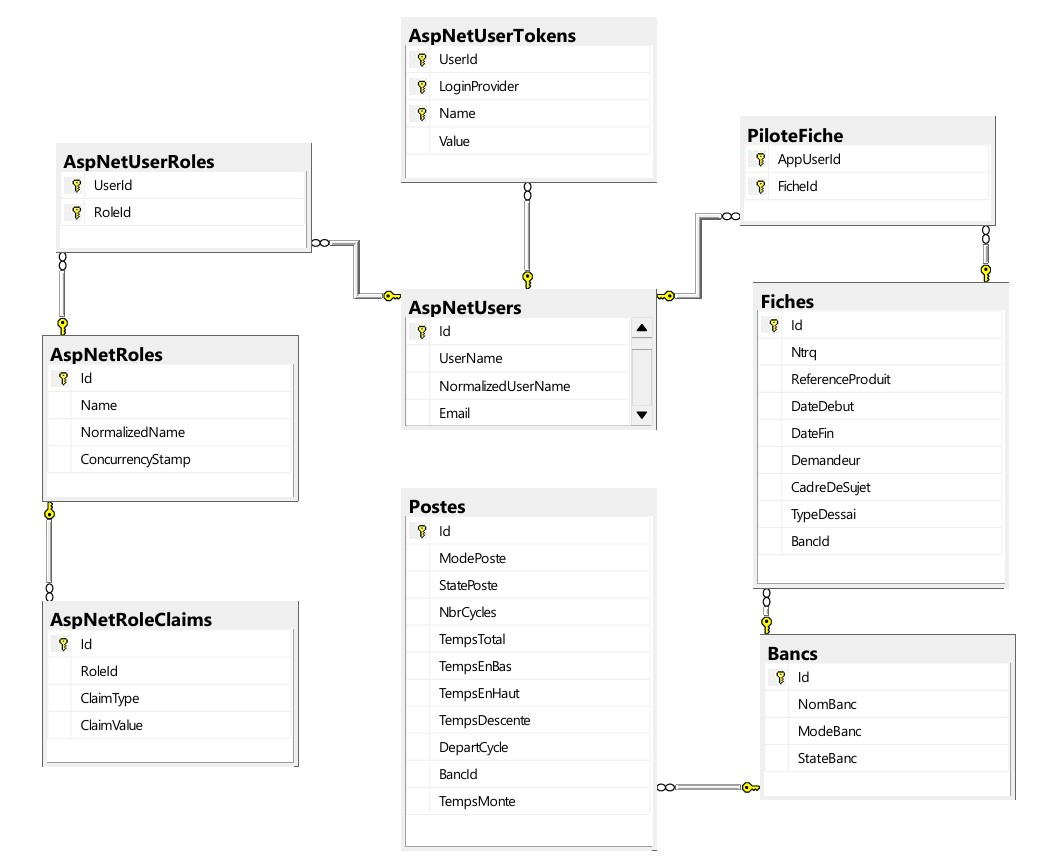
\includegraphics[width=1\textwidth]{chapters/3/img/16.jpg}
    \caption{cp 242-1 LEAN}
    \label{fig:campus}
\end{figure}


\subsection
{Services Déployés dans les iBox}
Pour récupérer les données des automates, plusieurs services ont été déployés sur les iBox :

\subsubsection{Service de Communication :} Gère les échanges de données entre les automates et les systèmes centralisés.
\subsubsection{Service de Stockage :} Assure la collecte et le stockage des données pour une analyse ultérieure.
\subsubsection{Service de Monitoring :} Surveille en temps réel les performances des automates et des flux de données.


\section{Communication and Data Integration}

\subsection{MQTT Protocol}
The MQTT protocol was chosen for its lightweight communication capabilities, particularly suitable for Industrial IoT environments. This enabled real-time updates between the lab equipment and the central system.
\begin{figure}[H]
    \centering
    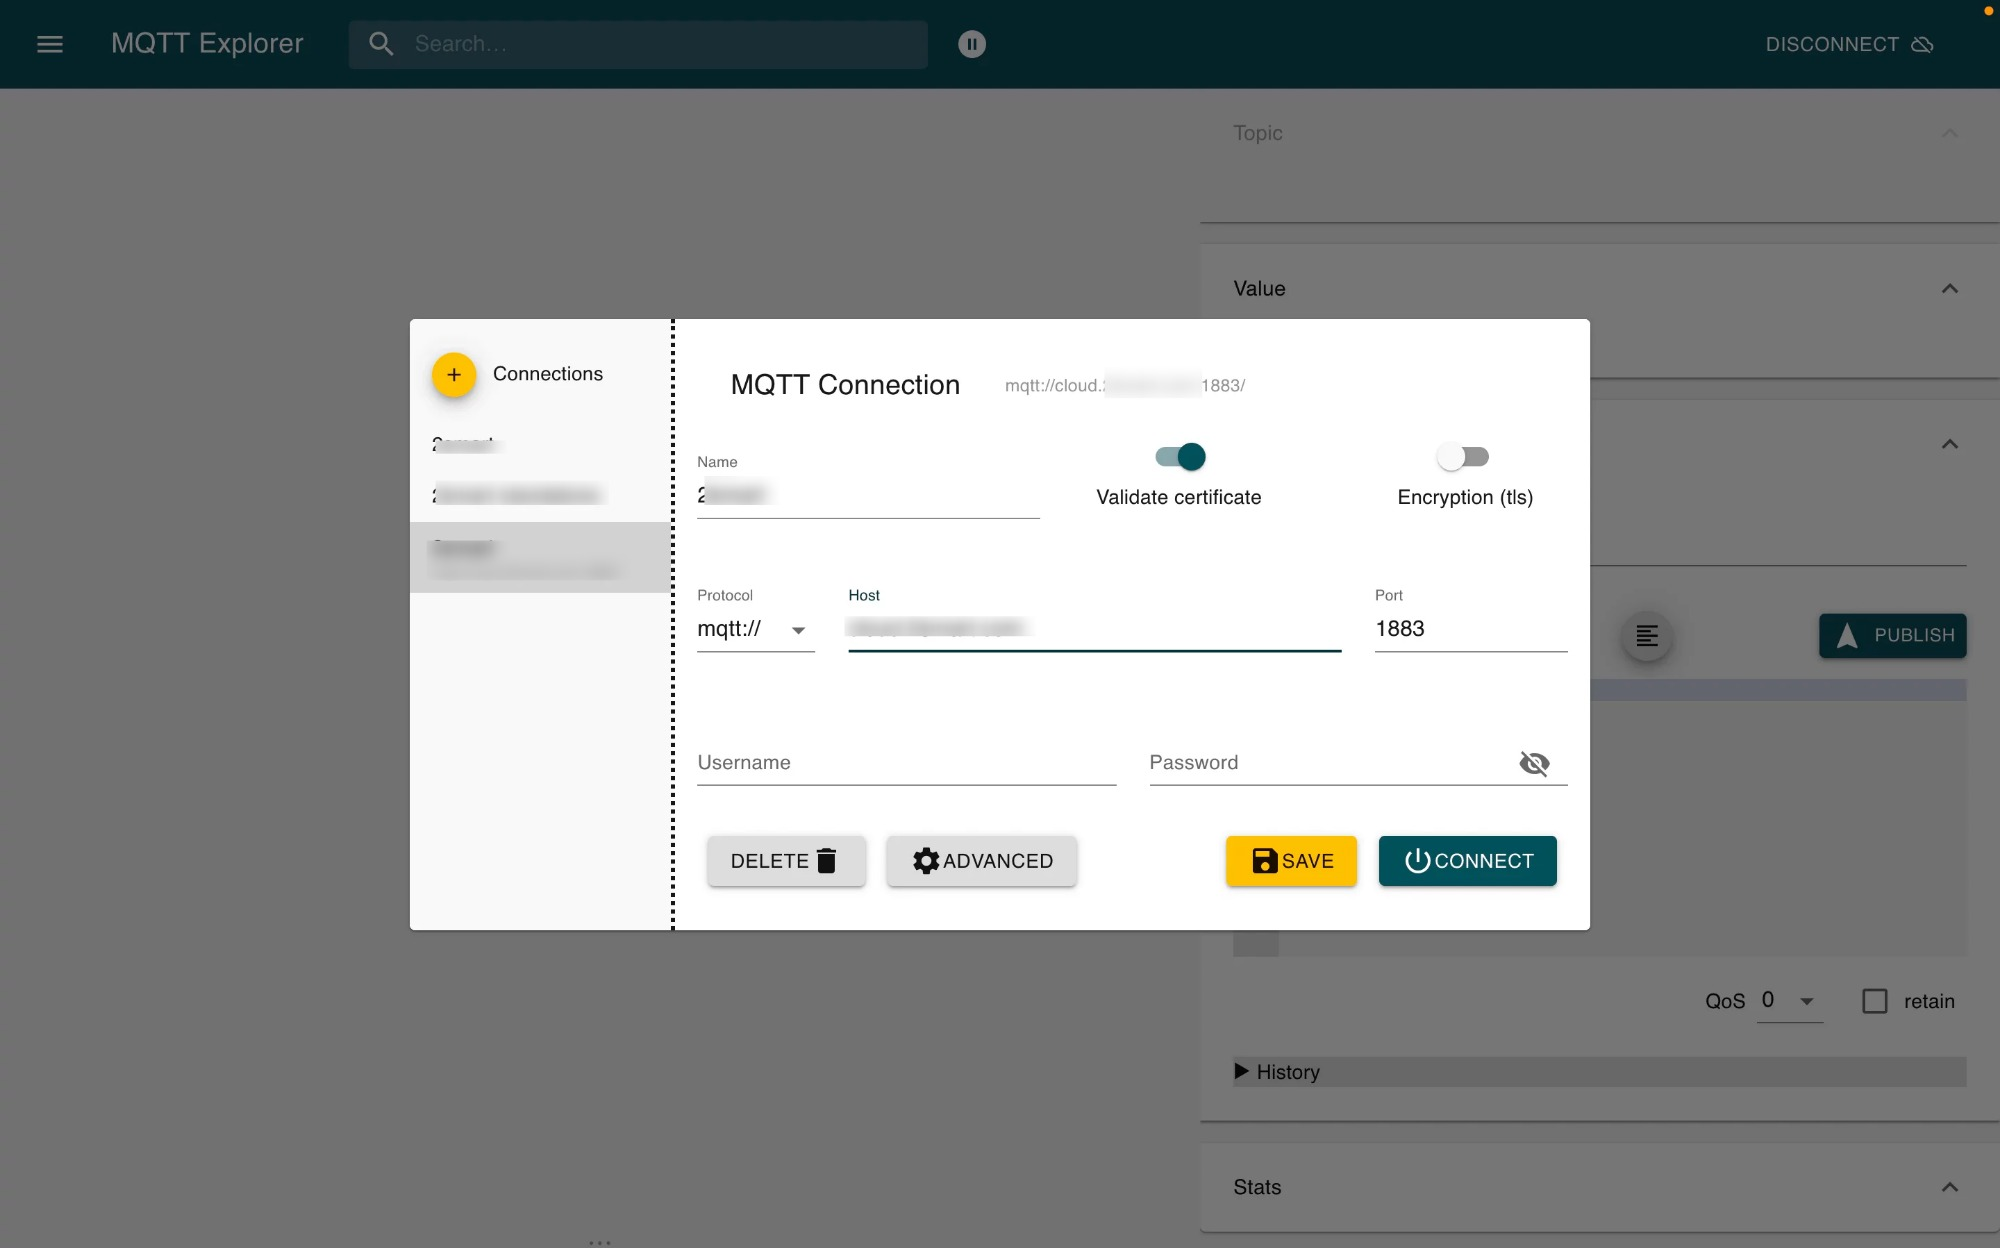
\includegraphics[width=1\textwidth]{chapters/3/img/15.jpg}
    \caption{cp 242-1 LEAN}
    \label{fig:campus}
\end{figure}
\begin{itemize}
    \item \textbf{Data Transmission}: Controllers publish sensor data to the MQTT broker, which is then consumed by backend services for processing.
    \item \textbf{Event-Based Architecture}: The platform reacts to changes instantly, ensuring timely updates and alerts.
\end{itemize}
\begin{figure}[H]
    \centering
    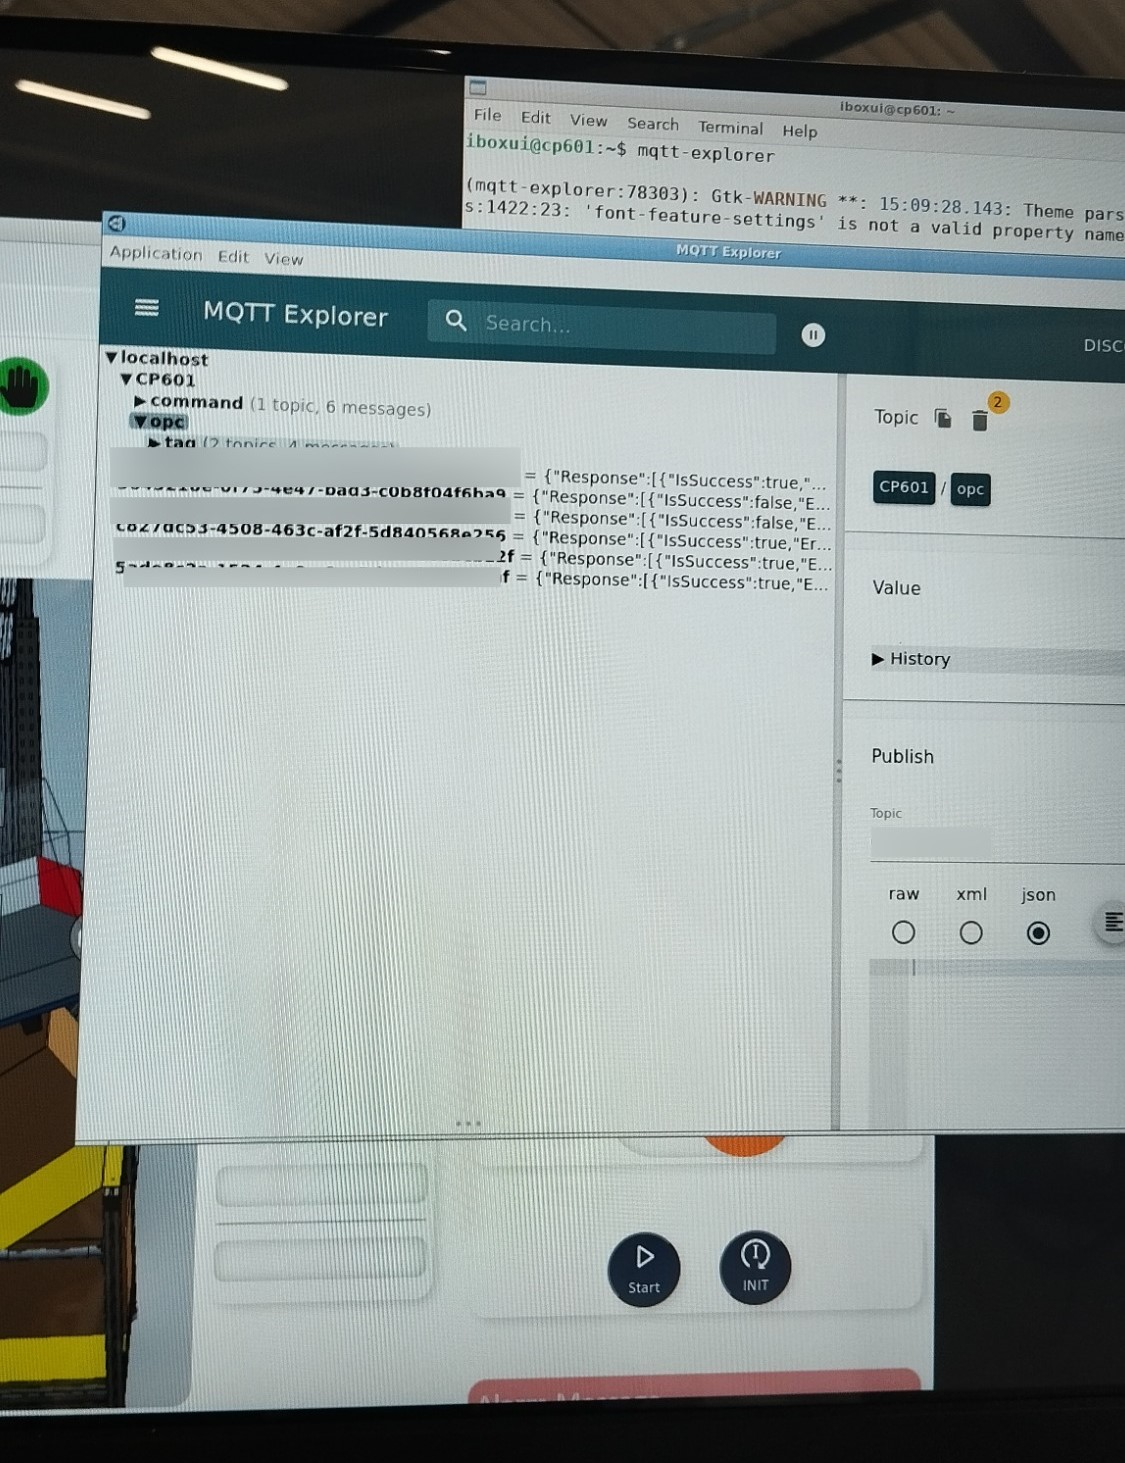
\includegraphics[width=0.6\textwidth]{chapters/3/img/14.jpg}
    \caption{cp 242-1 LEAN}
    \label{fig:campus}
\end{figure}


\subsection{Integration with Industrial Controllers (Step7 Siemens)}
The Siemens Step7 software was used to program controllers that manage laboratory equipment. The controllers were integrated with the LAB.E.S platform via MQTT, enabling automated data collection and control.


\section{IDE Step7 et Programme Automate}
IDE Step7 est l'environnement de développement intégré utilisé pour programmer et configurer les automates S7-300. Cet outil permet de créer des programmes d'automatisation complexes et de configurer les modules de communication.

Programme Automate et Modifications
Pour permettre la récupération des données en temps réel via le CP343-1 Lean, il a été nécessaire d'apporter des modifications au programme des automates. 

Les étapes incluent :
Configuration du CP343-1 Lean : Définition des paramètres réseau et des protocoles de communication.
Mise à Jour du Programme : Adaptation du code existant pour intégrer les nouvelles fonctionnalités de communication.
Tests et Validation : Assurer que les données sont correctement transmises et reçues.
\section{IDEs}

\subsection{Hardware}
\begin{figure}[H]
    \centering
    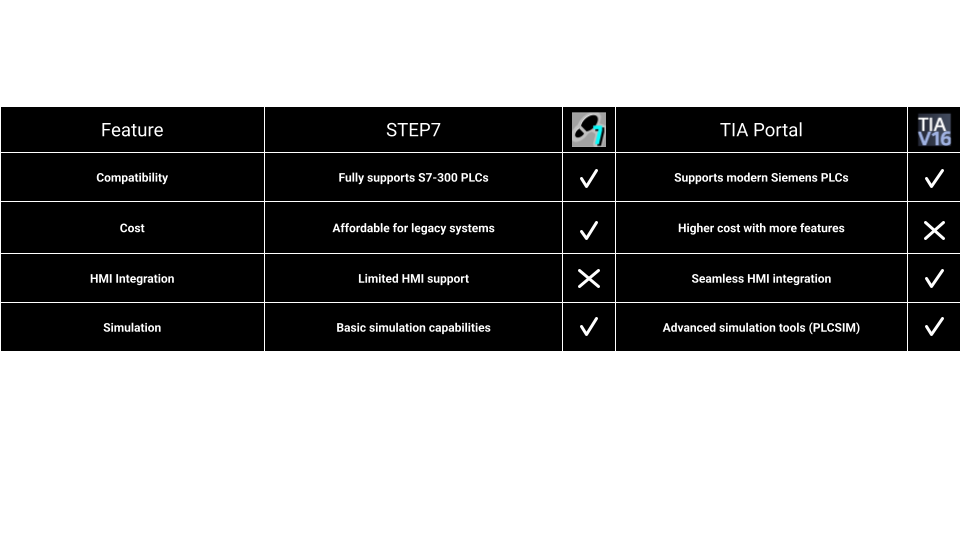
\includegraphics[width=1\textwidth]{chapters/3/img/101.png}
    \caption{cp 242-1 LEAN}
    \label{fig:campus}
\end{figure}

\subsection{UX/UI}
Ensuring real-time data synchronization between controllers and the platform was a challenge due to network latency. This was addressed by optimizing MQTT communication and implementing efficient data caching strategies.

\subsection{Back-end}
Ensuring real-time data synchronization between controllers and the platform was a challenge due to network latency. This was addressed by optimizing MQTT communication and implementing efficient data caching strategies.


\subsection{Fronted}
Ensuring real-time data synchronization between controllers and the platform was a challenge due to network latency. This was addressed by optimizing MQTT communication and implementing efficient data caching strategies.



